\documentclass[11pt,a4paper]{article}

\usepackage{tabulary}
\usepackage{tabularx}
\usepackage{booktabs}
\usepackage{array}
%\usepackage[dvips]{graphicx}
%\usepackage[longnamesfirst, round]{natbib}
\usepackage[round]{natbib}
\usepackage{graphics}
\usepackage[pdftex]{graphicx}
\usepackage{epstopdf}
\usepackage{epsfig}
%\usepackage{natbib}
%\biboptions{longnamesfirst,round,semicolon}
\usepackage{a4wide}
%\usepackage{mathptmx}
\usepackage{amssymb}
\usepackage{amsmath}
\usepackage{times}
%\usepackage[sidewaysfigure]{rotating}
\usepackage{float}
%\usepackage[latin1]{inputenc}        %f{\"u}r deutsche Texte
\usepackage[T1]{fontenc}             %f{\"u}r deutsche Texte
\usepackage{srcltx}
\usepackage{hyperref}
\graphicspath{{./figures2_3/}}
%\setlength{\parindent}{0pt} %keine Einrueckung erster Absatz
%\sloppy


\begin{document}

%\begin{center}
%COMMENTS ARE WELCOME - PLEASE DO NOT CITE
%\end{center}
%\begin{abstract}

%\end{abstract}
%\clearpage
%\tableofcontents
%\clearpage
%\listoffigures
%\clearpage

%%%%%%%%%%%%%%%%%%%%%%%%%%%%%%%%%%%%%%%%%%%%%%%%%%%%%%%%%%%%%%%%%%%%%%%%%%%
%\section{Appendix A: How to use the Modelbase software}
\begin{center}
{\Large \textbf{Macroeconomic Model Data Base 3.1 - User Guide } }
\par\end{center}


\vspace{1.5cm}


\noindent This user guide describes how to install and use the Macroeconomic Model Data Base, version 3.1 (hereafter the Modelbase or MMB). Section 1 deals with the installation and the software requirements.
Section 2 introduces the menu of the MMB 3.1 and describes how to run the software and conduct comparison exercises employing the models and options contained in the Modelbase.
Section 3 explains the structure of the key files that govern the simulations carried out by the MMB 3.1. Lastly, section 4 lays out the structure of the model files. These are usual Dynare files, which have been amended with extra lines and commands to suit the MMB.
For the time being we exclude instructions on how to alter the MMB by adding models or policy rules, which are planned to be included in the next release.

This guide is platform independent and can be applied to Windows, Linux and macOs operating systems.


%************************************************************************************
%
%
%   INSTALLATION
%
%************************************************************************************
%%%%%%%%%%%%%%%%%%%%%%%%%%%%%%%%%%%%%%%%%%%%%%%%%%%%%%%%%%%%%%%%%%%%%%%%%%%
\section{Installation and software requirements}\label{sec:installation}
\vspace{0.5cm}
The MMB 3.1 can be downloaded from \url{macromodelbase.com/download}. The version for windows is \texttt{mmb-electron-win.exe}, for macOS it is \texttt{mmb-electron-mac.dmg}, and for Linux directly download the source code from the release on github at
\url{https://github.com/IMFS-MMB/mmb-gui-electron/tags}.\footnote{Linux users will have to build from source using \texttt{npm}. Find more info on our github page.}
The Windows version and the Mac version of the file autoinstall the MMB on your computer and opens the redesigned frontend of the MMB. 

The files for carrying out the simulations of the models are written in MATLAB, so either some version of MATLAB or a recent version of its freeware clone, OCTAVE, must be installed on your computer. In the case of Matlab, one also needs the \textit{Optimization Toolbox} as well as the \textit{Statistics Toolbox} in order to be able to run all models in the Modelbase.\footnote{For the time being there are some models, which cannot be simulated with Octave. The list of models contains: NK\_GK11 and EA\_Q14. The problems with the latter model exist only with Octave 4.4.0.}.
For model solution the program utilizes DYNARE, which can be downloaded free of charge from the web.\footnote{\url{http://www.dynare.org}} Under Windows, double-clicking on the downloaded DYNARE exe-file opens a set of steps that guide you through the installation. Under macOS, locate the downloaded pkg-file in Finder, and Control-click the icon to select Open from the menu, thus creating an exception for the app to be installed. The installer will then guide you through the installation. To install Linux verison of Dynare please follow the instructions on the Dynare Wiki\footnote{The DYNARE Wiki install guide for Ubuntu and Debian can be found at \url{http://www.dynare.org/DynareWiki/InstallOnDebianOrUbuntu}}.

\subsection*{Compatibility}

REVISE THIS SECTION

We have tested the MMB 3.0 with DYNARE 4.5.6 and 4.5.7. Earlier versions may work but have not been tested.\\
On Windows, DYNARE 4.5.6 is compatible with OCTAVE 4.4.0, whereas DYNARE 4.5.7 is compatible with OCTAVE 4.4.1. Both Dynare versions are compatible with  MATLAB R2007b and later. For macOS, the compatibility between DYNARE and MATLAB is the same. However, at the time of this release, the highest OCTAVE-supported version of DYNARE is 4.5.6 (compatible with OCTAVE 4.4.0 on macOS).\\


\subsection*{Further steps before running comparisons}
When using MATLAB, one has to add the DYNARE path to MATLAB. In order to do so, open MATLAB and choose \textit{Set path} from the \textit{File} menu. Use the option \textit{Add folder} and browse to the directory where you have installed DYNARE. The DYNARE subfolder that has to be added is called \textit{MATLAB}.
When using OCTAVE, one adds the DYNARE path by opening the command window of OCTAVE (it should be open automatically) and typing "\textit{addpath directoryofdynare}". If you don't change the installation directory of OCTAVE you should type "\textit{addpath C:\textbackslash dynare\textbackslash 4.5.x\textbackslash matlab}", where x completes the version of dynare.   

%Before running simulations with the MMB, you need to specify whether you want to run the simulations in MATLAB or OCTAVE. In order to do so, click on settings on the upper-right corner of the MMB as shown in the Figure 'Settings'. 
Before running simulations with the MMB, you need to specify whether you want to run the simulations in MATLAB or OCTAVE. In order to do so, click on `Menu' on the upper-right corner of the MMB and then on `Settings', as shown in the Figure 'Settings'. It opens a window, in which you have the option either to let the program scan for versions of MATLAB and OCTAVE installed on your computer, or to search manually. If the scan finds more than one version of MATLAB or OCTAVE, you can choose from the list of programs in this subwindow by clicking on the small arrows on the right side. Note that the scan only looks in common directories as scanning the whole system would take too long. If the scan does not find the desired installation, click on `Find manually', select whether you want to add MATLAB or OCTAVE to the list of executables  and browse to the folder of the installation. Select the executable file which opens the program and click on `Open'. In case of MATLAB you should browse to "\textit{...\textbackslash matlab\textbackslash version\textbackslash bin\textbackslash matlab.exe}". Accordingly, for OCTAVE this is "\textit{...\textbackslash octave\textbackslash version\textbackslash bin\textbackslash octave-cli.exe}". If you want to remove an entry from the selection menu, select it and click on `Remove selected'.

You can follow the same steps  to select or delete a version of DYNARE on which you want to run the simulations.

Finally, the `Settings' menu also allows you to set a path of the MMB. You can either select a folder by clicking directly into the path field and extract the files shipped with the MMB into this folder by clicking on `Extract files'. You can also click on `Select folder' to choose a folder in which you already have installed the MMB. This option can be used if you have installed more than on version of the MMB, e.g. an original one and one in which you changed  or added models or policy rules. Thirdly, you can click on `Use builtin' to reset the folder and use the default MMB files shipped with user interface you are using.

To check whether your installations of MATLAB/OCTAVE and DYNARE are compatible with the MMB, click on `Check compatibility' in the lower left corner. This check can take up to 30 seconds. 

You can close the `Settings' window by clicking on `Close' in the lower right corner or on the cross in the upper right corner.

\begin{figure}[H]%[htb]
\centering
\caption{\textsc{Settings}}
\vspace{0.2cm}
\includegraphics[width=12cm,keepaspectratio]{settings31}\\[1cm]
\includegraphics[width=9cm,keepaspectratio]{settings2_31.png}
\label{img:Settings}
\end{figure}








%%%%%%%%%%%%%%%%%%%%%%%%%%%%%%%%%%%%%%%%%%%%%%%%%%%%%%%%%%%%%%%%%%%%%%%%%%%
\section{The Modelbase: Models, Rules and Options}\label{sec:usingMMB}
\vspace{0.5cm}
%\section{Using the MMB}
This section introduces the menu of models, policy rules and options, which can be selected in the MMB 3.1.
% For the time being, this version of the MMB does not feature the option of  model-specific shocks, and does not allow for flexible selection of the states and gain parameters used in the simulations of adaptive learning models. We will reintroduce these features into the MMB in the next release. 
\subsection*{Models}
For the time being there are some models, which cannot be simulated with Octave 4.4.0. The list of models contains: EA\_Q14. We will address these issues in the next release.

The user can select from the number of models displayed in the frontend, and from the number of policy rules. In contrast to earlier versions, the MMB 3.1 simultaneously allows for the selection of more than one policy rule and more than one model (the earlier versions either only allowed for one model, many rules or one rule, many models).  So, the user can select policy rules, shocks and variables, which are common in all selected models or remove common variables, which are automatically selected.

%\begin{figure}[H]
%	\centering
%	\caption{\textsc{Models and Rules Menu}}
%	\vspace{0.2cm}
%	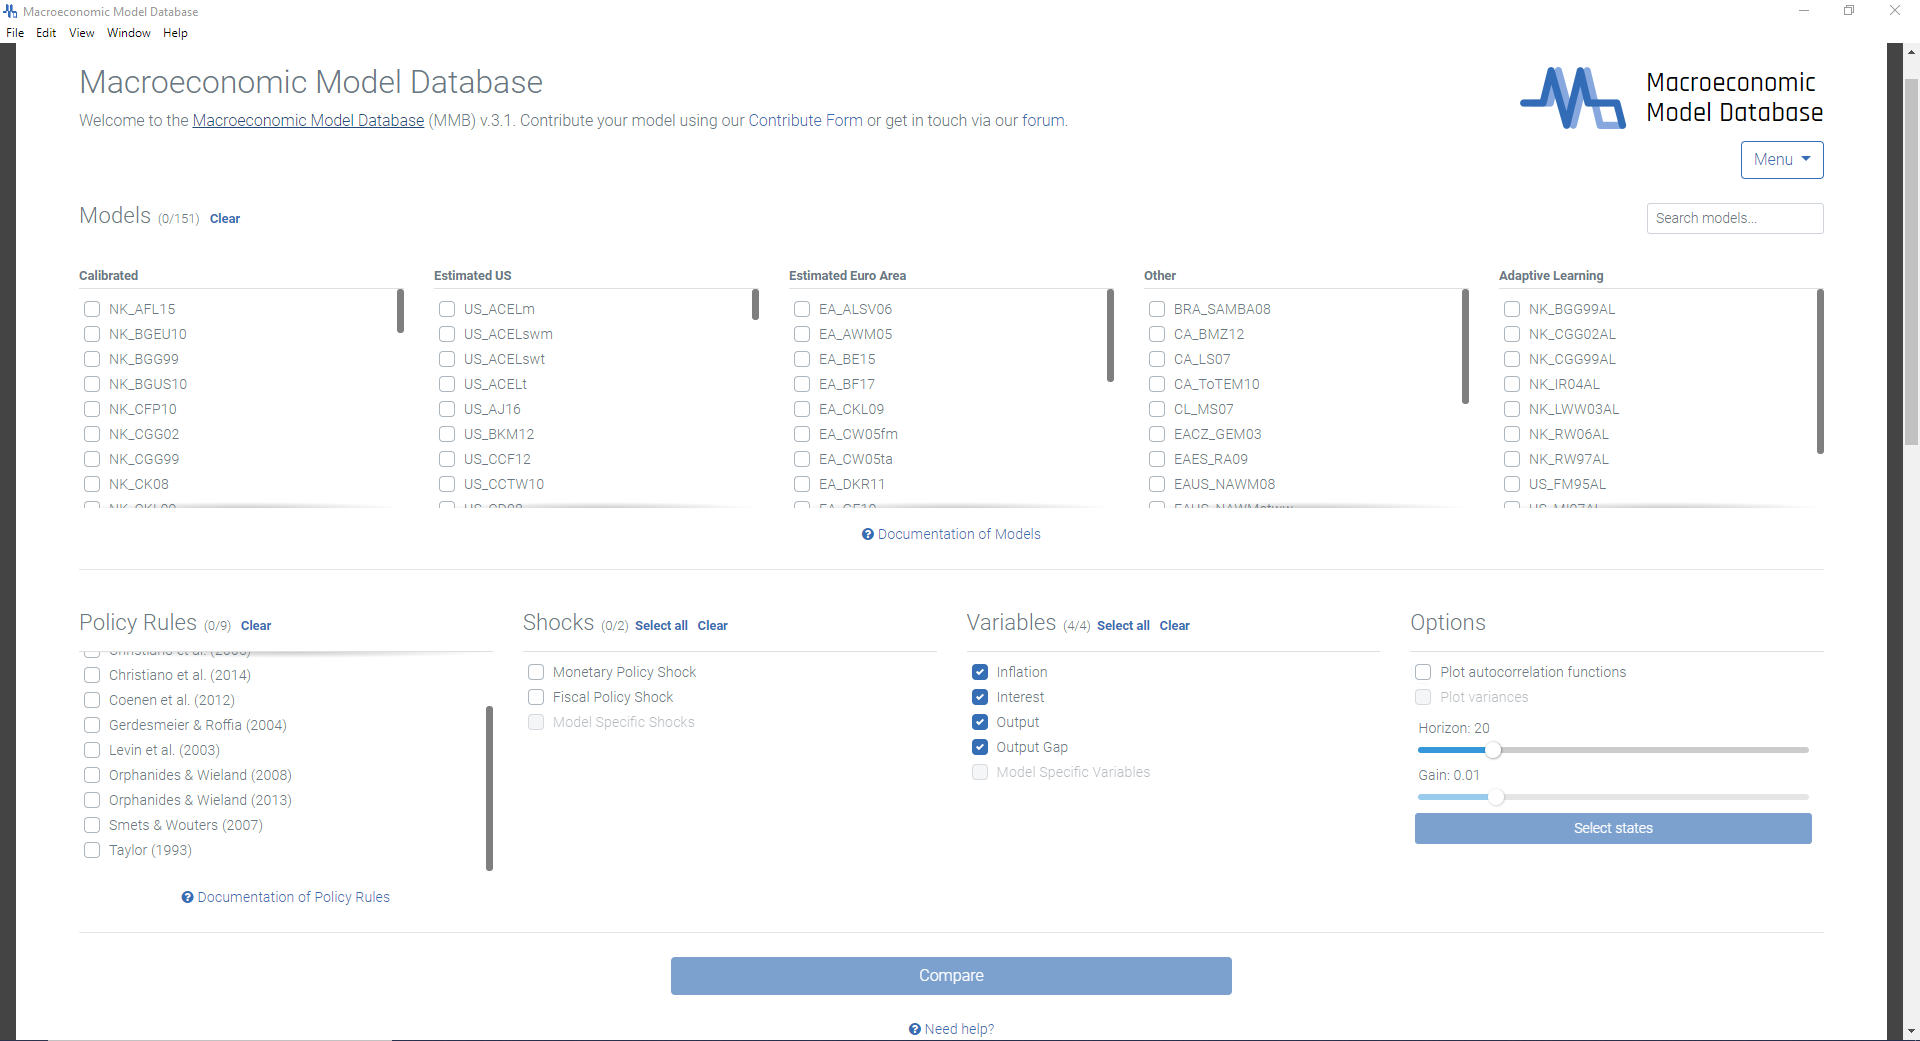
\includegraphics[width=15cm,keepaspectratio]{frontend.png}\\
%	\label{img:Models}
%\end{figure}

\begin{figure}[H]
	\centering
	\caption{\textsc{Models Menu}}
	\vspace{0.2cm}
	\includegraphics[width=15cm,keepaspectratio]{frontend_models31.png}\\
	\label{img:Models}
\end{figure}

The models are sorted in columns, the first of which contains models that have been calibrated to match a closed economy (NK\_xxx). The second column lists models that have been estimated on US data (US\_xxx). The third column lists models that have been estimated on Euro area data (EA\_xxx). The column 'Other' contains models that have been either calibrated or estimated on multi-country data, or have been estimated on other countries, such as 'CA\_BMZ12', which has been estimated on Canadian data, or 'EAUS\_NAWM08', which has been estimated on Euro area and US data in a two-economy-setting. The last column contains models in which agents form their expectations via adaptive learning (xxxAL). 
%\textbf{For the time being, until the options for the adaptive learning models are reintroduced into the MMB, all states are selected by default and the gain parameter is fixed to 0.01}. 


Hovering with the mouse over the models in the list and over the common policy rules displays some basic information such as the title, author and academic reference of the article, in which the model was used. To search for models in the MMB, one can also use the search line on top of the menu. Here one can search for the name of the author or words that appear in the title of the articles, in which the models were used as well as journals or year of publication. For instance, searching for Gal{\'\i}, yields the results shown in Figure \ref{search}.

\begin{figure}[H]
	\centering
	\caption{\textsc{Models Search: Gal{\'\i}}}
	\vspace{0.2cm}
	\includegraphics[width=15cm,keepaspectratio]{gali.png}\\
	\label{search}
\end{figure}

In addition, the user can download a complete list of all models currently used in the MMB on \url{macromodelbase.com/downloads}. Lastly, short descriptions of the models and their features are available on the same page. The menu of the MMB contains a direkt link to the model descriptions below the model selection menu as shown in Figure \ref{docmod}.
\begin{figure}[H]
	\centering
	\caption{\textsc{Model Documentation}}
	\vspace{0.2cm}
	\includegraphics[width=15cm,keepaspectratio]{documentmodels31.png}\\
	\label{docmod}
\end{figure}

\subsection*{Monetary policy rules}



Currently, we consider nine monetary policy rules that are taken from \cite{Taylor1993}, \cite{LevinWielandWilliams2003}, \cite{SmetsWouters2007}, among others. Next to these common rules that can (in principle) be used for all models, the selection menu also features the options model specific rule and user-specific rule. 
The model specific rules are taken from the original articles, in which the models were used. Not all models can be simulated with their model-specific rule, as all interest rate rules that can be used in the modelbase, have to be expressed in terms of the common variables. These common variables are the quarterly output gap, quarterly output, the year-on-year rate of inflation and the policy interest rate in annual terms. As some of the interest rate rules used in the literature feature responses to financial indicators, exchange rates, etc. these rules cannot be included in the modelbase. Therefore only 93 of the 128 models included in the MMB 3.0 feature a model-specific rule. 
%%%%%%%%%%%%%%%%%%%%%
%CHECK THESE NUMBERS%
%%%%%%%%%%%%%%%%%%%%%

\begin{figure}[H]
	\centering
	\caption{\textsc{Policy Rules Menu}}
	\vspace{0.2cm}
	\includegraphics[width=15cm,keepaspectratio]{frontend_pr31.png}\\
	\label{img:PR}
\end{figure}

The user specific rule allows the user to directly determine the feedback coefficients in the interest rate rule. In order to do so, the user has to click on `(edit)' next to the entry `User specific rule' as shown in figure \ref{img:PR}. Then, the subwindow shown in figure \ref{userrule} opens. In this example, the coefficients for current and lagged inflation rates, as well as for the current output gap are chosen such as to mimic the pre-programmed Taylor rule. The time indices refer to quarters. Click on `OK' to set the policy rule or on `Cancel' to discard changes.

The user can edit the coefficients of the responses of the policy rates to the leads and lags of the variables in this submenu. However, it is not guaranteed that the Blanchard-Kahn conditions will hold and a determined equilibrium is obtained in the solution of the models with this rule. 

\begin{figure}[H]
	\centering
	\caption{\textsc{Model Documentation}}
	\vspace{0.2cm}
	\includegraphics[width=15cm,keepaspectratio]{userrule.png}\\
	\label{userrule}
\end{figure}

In general, when a model (or a pre-specified rule) is chosen that is not compatible with a policy rule (or a model) in the way that a simulation of this model-rule-combination does not render the rational expectation equilibrium locally unique, the respective policy rule (or model) is faded out in the menu and cannot be selected for the comparison exercise. Unselecting the model (or rule), makes the rule (or model) again accessible for selection. 

\subsection*{Output options}

Having chosen the models and a policy rule, the user can make some non-exclusive choices regarding the exercise outcomes to be displayed.
The user can decide whether to see the unconditional variances and plot autocorrelation functions of the common variables, both of which are computed using theoretical moments of the solution for each variable. Also the user can opt for plotting impulse response functions of the common variables and specify the horizon for the analysis that is set to twenty periods as a default. 

As default the common MMB variables (quarterly output gap, quarterly output, the year-on-year rate of inflation and the policy interest rate in annual terms) are selected. If only one model is chosen, all other variables as defined in the mod-file are also available. As a new feature in the MMB 3.1, some more variables which are featured in many of the models, but not in all of them  (among others consumption, investment and capital) can be selected for comparison if available in all selected models. 

One can choose impulse responses to a unit monetary policy shock (one percent point increase in the monetary policy shock), and/or to a unit fiscal policy shock (one percent increase in GDP share of government expenditures). Note that all models of the Modelbase have a monetary policy shock, but a significant number of them do not have a fiscal policy shock. If this is the case, the impulse responses to a fiscal policy shock will not be available. Again, if only one model is selected, all model-specific shocks as defined in the mod-file are available for selection. Alongside the new comparable variables, also a number of shocks  appearing in many models are now available for comparison (e.g. Technology shock, Preference shock).
%AL

When you select an adaptive learning model, you can also set the gain parameter and select the states by clicking on `Select states'. In the window that pops up you can select the states individually for all adaptive learning models you have selected for the comparison.

Lastly, for certain models, the unconditional variances are not defined and the autocorrelation functions do not exist. This is the case for some models which feature unit roots. The presence of unit roots prevents a calculation of unconditional moments of some or all variables. Nonetheless, for these models IRFs can still be generated. 


\subsection*{Menu}
In the upper right corner of the MMB GUI you can find the button `Menu'. When clicking the button, a drop-down menu opens, where you can click four buttons.\\
Firstly, `Edit Rules/Models' opens a sub-window with all models included in the MMB. Here you can manually find the model you want to edit. After clicking on a model name, you can see its two relevant files, namely the .json and .mod file. The .json file contains basic information about the model, like paper title, author and journal, but it also contains information about the model capabilities, i.e. if the model is capable of producing the common variables (output, inflation, interest rate, output gap) and common shock (monetary and fiscal policy shock). As an example, \textit{fiscal\_shock": false} means that the model does not contain a fiscal policy shock. You can also see if unconditional variances are possible for this model and if it is an adaptive learning model. Furthermore, under \textit{rules} you can see which policy rule is eligible for the model you want to edit, while under \textit{msr} you can see and change the coefficients for the model specific policy rule. In the block below, you can see the name and the text of each shock and below that of each variable contained in the model. In case you want to change the name of a shock or variable appearing in the main-window, please change its text to the desired text. Hint: The text is case sensitive, so if you want to change the name of a variable for many models, be consistent with the text. The other file appearing in for the selected model is the .mod file. This file consists of a preamble defining all variables, shocks and parameters. It is followed by the parameter initialization and the model equations, which define the sticky price and wage economy and the flex economy, as well as shocks. In the case of non-zero steady state values of variables, there usually also exists a separate \textit{modelname\_steadystate.m} file, which defines the steady state of the model. In the upper right corner of the sub-window you can save the changes of the current file. It is important to keep in mind that you need to save the file before switching to another file because then unsaved changes are gone. Also, saving the changes does not apply them. You need to reload the data. At any time you can close the sub-window by clicking the `Close' button in the lower right corner of the sub-window. 
%There is no folder with policy rules, only models

The second button in the drop-down menu is `Reload Data' and applies the saved changes made to the files, i.e. renaming a shock or variable.
%%%%%%%%%%%%%%%%%%%%%%%%%%%%%%%%%%%%
%Maybe problem here (when renaming)%  
%%%%%%%%%%%%%%%%%%%%%%%%%%%%%%%%%%%%

The third button `Settings' is explained in section \ref{sec:installation}.

The last button `Help' opens a help window. 


\subsection*{Running a comparison exercise}
Once you have selected a number of models, rules and output options, you can simply run the comparison exercise by clicking on the button `Compare'. When the simulations run the command window from MATLAB/OCTAVE will be embedded and you see the running output (see, Figure \ref{mmbsimul}). Once the simulations are finished you can close the window by clicking on `Close'.
%If you have chosen to run your simulations using OCTAVE, the command window from OCTAVE will be embedded and you see the running output (see, Figure \ref{mmbsimul}). If you are using MATLAB, a second window opens, in which the simulations are displayed as in MATLAB's command window. This second window closes automatically when the simulations are done.
 
\begin{figure}[H]
	\centering
	\caption{\textsc{Model Simulation}}
	\vspace{0.2cm}
	\includegraphics[width=15cm,keepaspectratio]{mmbsimul.png}\\
	\label{mmbsimul}
\end{figure}

As a result, the selected Impulse response functions and  autocorrelation functions are plotted, and the variances are displayed in a table at the bottom of the frontend. 
There are different options available to display the results (see figure \ref{display}). First, the user can choose whether results should be displayed in charts of variables, models or policy rules. This can be selected by clicking on `Group Data' and then the respective option. The default is to group outputs by variable, i.e. the charts represent variables and the graphs in the charts represent model/policy rule-combinations. 
Further, the user can select the `maximum number of columns per row', which might be useful to increase readability or clarity depending on the screen used. 
Finally, the user can choose which graphs are displayed in the charts by clicking on the respective entries of the caption.

\begin{figure}[H]
	\centering
	\caption{\textsc{Display Options}}
	\vspace{0.2cm}
	\includegraphics[width=15cm,keepaspectratio]{display31.png}\\
	\label{display}
\end{figure}


The results of the comparison exercise can be exported and saved in two ways. Either, one exports all the data, by clicking on CSV or JSON above the figures to receive a batch export in the respective file format, or one can export the figures one by one, by clicking on the menu on the upper right corner of each figure. Both options are marked with red boxes in Figure \ref{export}.
\begin{figure}[H]
	\centering
	\caption{\textsc{Export Options}}
	\vspace{0.2cm}
	\includegraphics[width=15cm,keepaspectratio]{export.png}\\
	\label{export}
\end{figure}


%%%%%%%%%%%%%%%%%%%%%%%%%%%%%%%%%%%%%%%%%%%%%%%%%%%%%%%%%%%%%%%%%%%%%%%%%%%
\section{Structure of the Modelbase}
\label{sec:MMBstructure}
\vspace{0.5cm}
This section describes the key folders, in which the models, options, and rules are stored and briefly sketches the structure of the key files, which are used in the execution of the modelbase.

\subsection*{Key Folders}
 
Your installation of the MMB 3.1 contains a subdirectory 'resources/app/dist/electron/static/mmci-cli', which contains the .m-files and .mod-files for the models, rules and options being used in the comparison exercises. 
The subfolder \textit{MODELS} contains a specific folder for every model included in the MMB. The specific folders contain a  DYNARE mod-file in which the particular model is specified together with related MATLAB files, some of which are created by DYNARE, as well as a json-file, which is needed to link information displayed in the user interface to the corresponding mod-file. 

The subfolder \textit{RULES} contains json files for each monetary policy rule.

The subfolder \textit{ALTOOLS} in the folder \textit{LIB} contains scripts for the use of models with adaptive learning. 

\subsection*{Some key files}
In earlier versions, the MMB had the subfolder \textit{MMB\_OPTIONS} containing specific MATLAB files related to the usage of the Modelbase for policy analysis and comparison, as well as explanatory notes for models and policy rules. These folders have been removed. The information is mostly contained in the .json file in the models folder.   

The files discussed here are stored in the folder MODELS and are a brief introduction. For further information read section \ref{sec:ModelfileStructure}.

\begin{itemize}
\item \textbf{modelname.mod}\\
This file contains the model variables, shocks and parameters as well as the model equations including the flex economy, the sticky price and wage economy and shocks. If the model is not linear, then sometimes the file also contains an \textit{initval} block, which provides guess values for non-linear solvers and steady state computations.
\item \textbf{modelname.json}\\
This file contains information about the capabilities of the model. It defines, which of the policy rules, the four common variables and two common shocks are eligible for this model. It also states if unconditional variances can be calculated. Additionally, the file contains general information about the model (e.g. paper, author,...). The model specific policy rule is included if it is available and also contains the exact parameter values. It is also stated if the model includes adaptive learning and if so it shows which variables are forwards, states\_short and states\_long. For all models, the name and text of all shocks and variables can be seen and changed in this file.
\item \textbf{optional: modelname\_steadystate.m}\\
In case of non-zero steady states, this file is included in the model specific folder and contains the steady state equations or values. 
\end{itemize}




%%%%%%%%%%%%%%%%%%%%%%%%%%%%%%%%%%%%%%%%%%%%%%%%%%%%%%%%%%%%%%%%%%%%%%%%%%%
\section{Structure of the model files}\label{sec:ModelfileStructure}
\vspace{0.5cm}
\subsection*{Mod files}
The model files are written in the syntax of DYNARE and have a common structure.
As an example we take the simple New-Keynesian model by \cite{RotembergWoodford1997} to
explain the structure of the mod-files, its model specific parts and the common model data base blocks. The current example is based on the DYNARE 4.5.6 version of the Modelbase. The mod-file is shown in {\bf Figure \ref{img:modStructureRW97a}} and {\bf Figure \ref{img:modStructureRW97b}}. However, the explanations apply to all models.
In the following, the two main parts of a mod-file, the preamble and the model block, are described step by step.

\begin{figure}[p]
\centering
\caption{\textsc{Structure of the model files: The Preamble}}
\vspace{0.2cm}
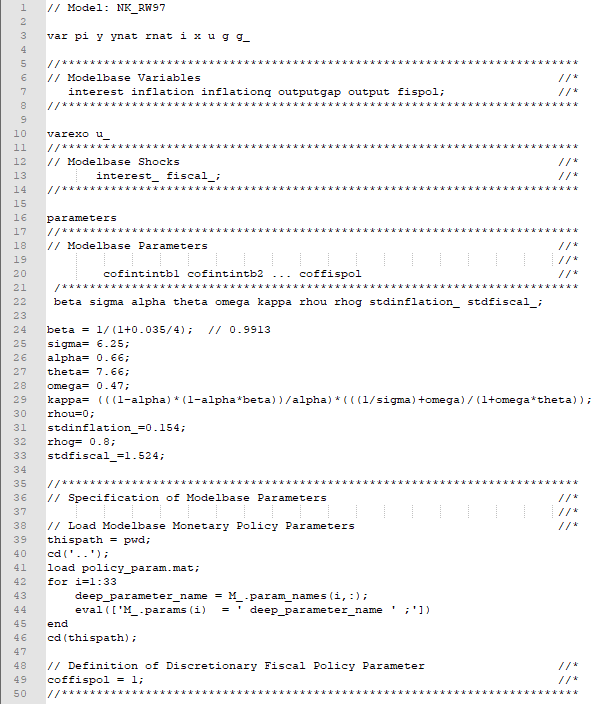
\includegraphics[width=15cm,keepaspectratio]{mod1.png}\\
\label{img:modStructureRW97a}
\end{figure}

\begin{figure}[p]
\centering
\caption{\textsc{Structure of the model files: The Model Block}}
\vspace{0.2cm}
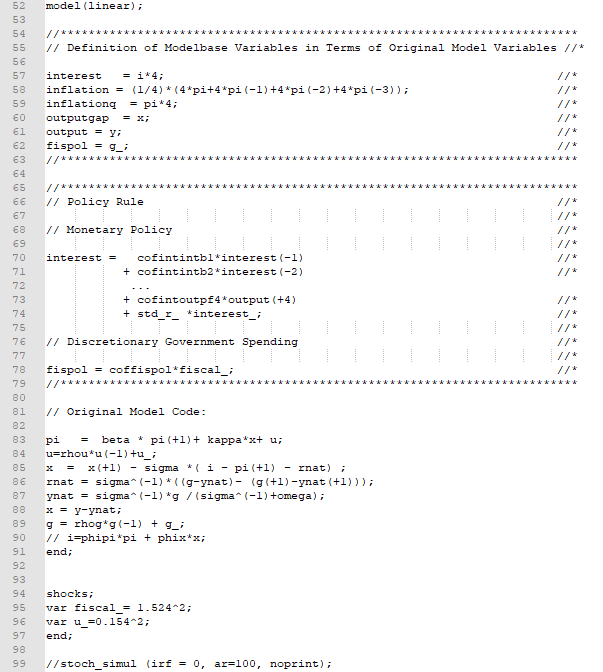
\includegraphics[width=15cm,keepaspectratio]{mod2.png}\\
\label{img:modStructureRW97b}
\end{figure}

\vspace{2cm}

\noindent {\it Part 1: The preamble}

\begin{itemize}
    \item Each model file begins with some information about the model. This should include the
    title, the authors, the publication etc. In front
    of this description you will find the symbols \textit{//}, which denote a comment in DYNARE.
    \item The file then starts with the initialization of the model variables. In our example shown in {\bf Figure
    \ref{img:modStructureRW97a}} the model-specific endogenous variables are listed in line 3 after the keyword \textit{var}:
    \textit{pi}, \textit{y}, \textit{ynat}, \textit{rnat}, \textit{i}, \textit{x}, \textit{u}, \textit{g}
    and \textit{g\_}. The latter in fact represents an exogenous government spending shock, however it has to be
    initialized as endogenous variable for reasons that will be explained below.
    It follows a Modelbase block in lines 5 to 8 in which the common variables are introduced.
    In general, Modelbase blocks are separated through \textit{//*******} symbols from the rest of the file.
    \item Following the keyword \textit{varexo} in line 10 the exogenous variables are initialized.
    In our example this is \textit{u\_}, a cost push shock as well as the common interest rate shock, \textit{interest\_} and
    the common fiscal policy shock, \textit{fiscal\_} in line 13. Note that in some models with no treatment of government spending, the
    latter Modelbase shock may be left out.
    \item Following the keyword \textit{parameters} in line 16, the Modelbase parameters in the Modelbase block are initialized.
    In {\bf Figure \ref{img:modStructureRW97a}} line 20 we have, for brevity reasons, only included three policy parameters.
    In the actual mod-files there are many more leads and lags. These are the parameters of the
    general monetary policy function, except for the last one, \textit{coffispol},
    which enters the common discretionary government spending equation.
    \item Then the model-specific parameters are initialized in line 22.
    \item Afterwards numerical values are assigned to the model-specific parameters in lines 24 to 33.
    \item Finally a block called \textit{Specification of Modelbase Parameters} is added. First in lines 38 to 46 the numeric
    values of the parameters of the selected monetary policy rule are loaded.
    They are contained in the file \textit{policy\_param.mat} in the subfolder \textit{MODELS}.
    For models in which the original shocks are expressed in percent/100 the parameter \textit{std\_r\_} has to be reset to 100
    after the parameter-loading command. In our example this would have to be done in line 45. However, the shocks in this model are
    already expressed in percentage terms. Secondly, the discretionary fiscal policy parameter \textit{coffispol} is defined as a function
    of the model-specific parameters in order to obtain a government spending shock of one percent of GDP. The exact
    implementation of the common fiscal policy shock will be described below. In our example no adjustment is
    needed and hence \textit{coffispol} is set equal to one.
\end{itemize}


\noindent {\it Part 2: The model block}

\begin{itemize}
\item The model block starts in line 52 of {\bf Figure \ref{img:modStructureRW97b}} as indicated by the keyword \textit{model} followed
by \textit{linear}, which tells DYNARE that the equations are already linearized and thus reduces computing time.
\item In the Modelbase block going from lines 54 to 63 the common variables are defined in terms of the original model variables.
The variable \textit{interest} denotes the annualized short-term interest rate, \textit{inflation} is annual inflation,
\textit{inflationq} represents annualized quarterly inflation, \textit{outputgap} and \textit{output} denote the output gap and output, respectively.
The common variable \textit{fispol} represents discretionary fiscal policy. It is set equal to the model-specific government spending
shock variable, which in the case of our example is \textit{g\_}. Note again, that this model-specific shock has to be initialized
as an endogenous variable. This allows us the keep the original model equation for government spending unchanged.
\item It follows the common \textit{Policy Rule} block. In lines 70 to 74 the common monetary policy rule is specified.
Again for reasons of brevity we have not displayed the complete general policy rule in {\bf Figure \ref{img:modStructureRW97b}}.
Below in line 78, the common equation for discretionary government spending is specified.
\item The original model equations are then specified in lines 83 to 90. Note that the model-specific monetary policy rule is commented out because the common policy rule is introduced. On the contrary, the government spending equation in line 89 has remained unchanged.
The model section ends in line 91 with the required keyword \textit{end}.
\item Finally the variance covariance matrix is specified in lines 95 and 96 between the keywords \textit{shocks} and \textit{end}. Importantly, the variance of the original model-specific government spending shock has been assigned to the common fiscal policy shock variable \textit{fiscal\_}. Hence, the common shock \textit{fiscal\_} affects the fiscal policy variable \textit{fispol} through the common discretionary government spending expression in line 78 which is set equal to the model-specific government spending shock \textit{g\_} in line 62.
\item The \textit{stoch\_simul} command in line 99 is commented out. Alternatively one can also delete this command.
\end{itemize}

\subsection*{Json files}
The json files have a common syntax. As take the same example as above to explain the structure of the json files. It can be seen in figure \ref{img:jsonstructure}.

Every json file starts with a curved bracket. All objects need to be specified in " ". Firstly, it is specified what the json file includes, here it is a model, followed by the name of the model (\textit{NK\_RW97}). Here, the first letters determine which type of model it is (e.g. New Keynesian model: NK, Euro Area: EA, United States: US, or others), followed by a `\textit{\_}'. The next letters are set according to the last names of the authors (here: RW stands for Rotemberg and Woodford). The name is completed by the year of publication (97 stands for 1997, while 03 or 13 stands for 2003/2013). Optionally, AL is added to the model in case the model includes adaptive learning. 

The first block you need to specify are the \textit{"capabilities"} (lines 4-22). It defines, which of the four common variables and two common shocks are eligible for this model. If they are included, the value is set to \textit{true}, else it is set to \textit{false}. After that \textit{"rules"} contains all policy rules, which are available for this model. Note that the set of available rules is written in square brackets. All unavailable policy rules appear in gray in the GUI and can not be chosen. In step 3 of section \ref{sec:HowToAddModels} there is a list showing which rule number belongs to which monetary policy rule. In the json file it also states if unconditional variances can be calculated (line 21). So for NK\_RW97, all common variables, shocks as well as unconditional variances are available. Rules 3-7 and 9-11 can be chosen. 

The next block, \textit{"description"} (lines 23-36), contains general information about the model, like reference, paper title, journal and year published, replicants name, keywords, description, category and authors. Again all sets are written in square brackets. This includes key words and authors. General information is shown when holding the mouse over a model. It is important to specify the category of the model because it specifies in which model block the model appears in the GUI. Type \textit{"Calibrated model"} for calibrated models, \textit{"Estimated euro area model"} for EA models, \textit{"Estimated US model"} for US models, \textit{"Estimated other-country model"} for other countries or \textit{"Adaptive learning model"} for adaptive learning models. Note that these entries are case sensitive.

\begin{figure}[H]
	\centering
	\caption{\textsc{Structure of the json files}}
	\vspace{0.2cm}
	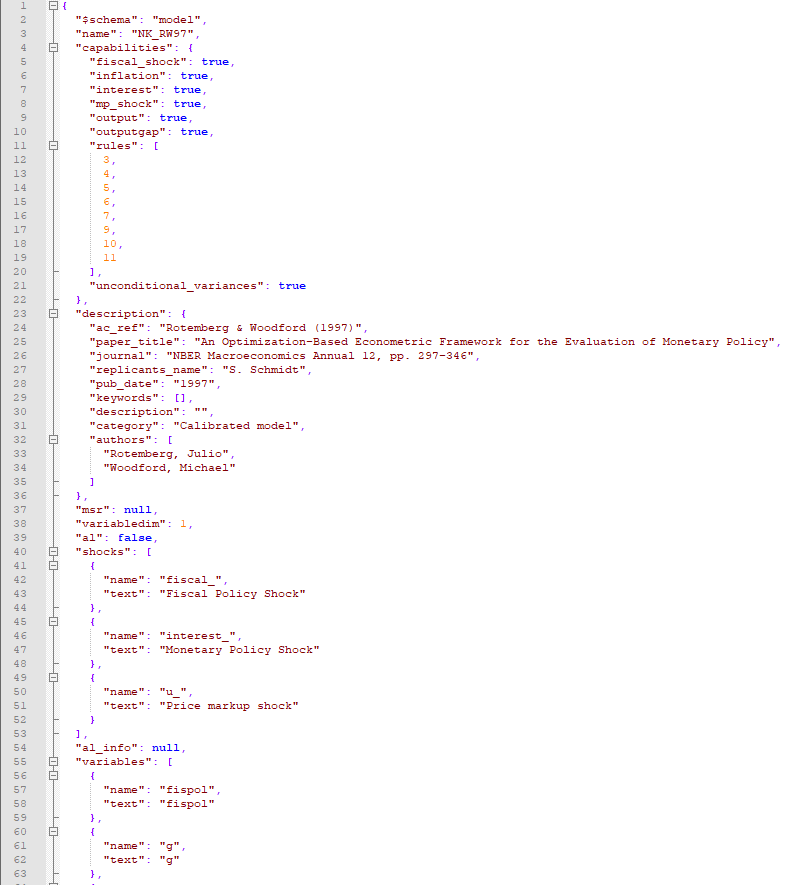
\includegraphics[width=15cm,keepaspectratio]{json1.png}\\
	\label{img:jsonstructure}
\end{figure}

Next, there is a block for the model specific policy rule. The New Keynesian model by Rotemberg and Woodford does not have a model specific policy rule, so this entry is set to \textit{null}. It is the policy rule used in the paper. Consider NK\_CGG02AL as an example for msr and adaptive learning. Figure \ref{img:jsonmsr} (left) shows the syntax for the msr entry. As it is a set, you need to specify the policy rule coefficients inside of square brackets.
%%%%%%%%%%%%%%%%%%%%%%%%
%which belong to which?% 
%%%%%%%%%%%%%%%%%%%%%%%% 

\begin{figure}[p]
	\centering
	\caption{\textsc{Structure of the json files: msr (left) and AL (right)}}
	\vspace{0.2cm}
	\begin{minipage}{.45\textwidth}
		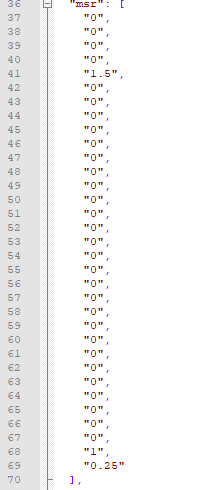
\includegraphics[keepaspectratio]{jsonmsr.png}\\
	\end{minipage}
	\begin{minipage}{.45\textwidth}
		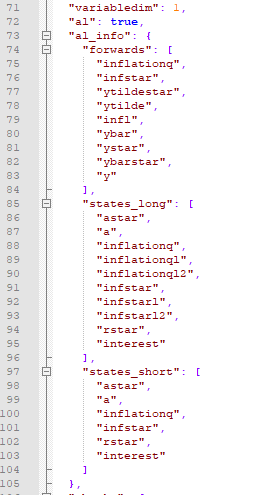
\includegraphics[keepaspectratio]{jsonal.png}\\
	\end{minipage}
	\label{img:jsonmsr}
\end{figure}

Afterwards, the dimension of the shock is specified using \textit{"variabledim"}. It is set to 1 if the shock is in percent, so the number 1 next to the graph means 1\%, and 2 if it is in percent/100. In this case the number 1 next to the graph would mean 0.01\%. However, MMB 3.1 takes this into account and standardizes it to \%.
%%%%%%%%%%%%%%%%%%%%%%%%%%%%%%%%%%%  
%Like this or the other way round?%
%%%%%%%%%%%%%%%%%%%%%%%%%%%%%%%%%%%

The next block is \textit{"al"}, in which adaptive learning properties are specified. If the model does not include this feature, then the entry is set to \textit{false}. Otherwise, it is set to \textit{true}. Figure \ref{img:jsonmsr} (right) shows the structure of the code in the case of adaptive learning. In this case \textit{"al\_info"} is added, which contains three features, namely \textit{forwards}, \textit{states\_short} and \textit{states\_long}. All of these features are a set of variables. 
%%%%%%%%%%%%%%%%%%%%%%%%%%%%%%%%%%%%%
%Features, states_short, states_long%
%%%%%%%%%%%%%%%%%%%%%%%%%%%%%%%%%%%%%

Lastly, there are blocks for \textit{"shocks"} and \textit{"variables"}, in which all shocks and variables of the model are listed. As the two objects are lists, the user needs to use square brackets. Every entry in the list is in curved brackets and separated by a comma. An entry contains a name and a text. The name is the same as in the mod file, while the text appears in the GUI. Note that the text is case sensitive.

%%%%%%%%%%%%%%%%%%%%%%%%%%%%%%%%%%%%%%%%%%%%%%%%%%%%%%%%%%%%%%%%%%%%%%%%%%%
\section{Adding models to the Modelbase}%\label{sec:HowToAddModels}
\vspace{0.5cm}
Adding a new model to the data base consists of four steps. First, the original model has to be translated into a DYNARE mod-file and the common Modelbase variables have to be defined as functions of the original model variables. Second, the mod-file must be stored under the model name in a folder with exactly the same label. Third, a json-file, which builds the link between the mod file and the GUI, has to be created. It also has to have the same  name and be stored in the same folder. The folder with both files has to be stored in the subdirectory `resources/app/dist/electron/static/mmci-cli/models'. Fourth, the GUI needs to be reloaded to incorporate the new model.
%Third, the new model has to be initialized in the Modelbase interface.  {\bf Figure 9} illustrates the Modelbase folders and in red we attract attention to the folders/files where one should initialize the new model. In the following, each of these steps is described in detail. \\

%\begin{figure}[H]
%\centering
%\caption{\textsc{Adding models in the Modelbase}}
%\vspace{0.2cm}
%\includegraphics[width=15cm,keepaspectratio]{../figures2_3/12addmodel.jpg}
%\label{img:MenuStructure6}
%\end{figure}

\noindent {\it Step 1: Creating the mod-file}

\begin{itemize}
\item The first task when adding a new model to the Modelbase is to create a DYNARE mod-file. The file should start with a comment section giving some information about the associated reference paper(s) for the model.
\item The file must have the usual structure of a DYNARE mod-file. That is, one starts with the initialization of variables, shocks and parameters. Then the equations describing the model follow and finally the variance-covariance structure of the shocks is specified.
\item However, each of the sections mentioned before has to be augmented by a Modelbase block. This Modelbase block should be visually separated from the original model sections through a comment line \textit{//*******}.
\item After the initialization of the original model variables, the common block \textit{Modelbase Variables} follows. It consists of the six common variables \textit{interest}, \textit{inflation}, \textit{inflationq}, \textit{outputgap}, \textit{output} and \textit{fispol}. Those variables will be described below. If output is not specified in the model, then the common variable \textit{output} has to be left out. Furthermore, in some small models, one may have to leave out the \textit{fispol} variable. This common block corresponds to lines 4 to 7 in {\bf Figure \ref{img:modStructureRW97a}}
\item The common block \textit{Modelbase Shocks} is added after the initialization of the original model shocks as in lines 10 to 13 of {\bf Figure \ref{img:modStructureRW97a}}. It consists of a common monetary policy shock, \textit{interest\_}, and of a common fiscal policy shock, \textit{fiscal\_}.
\item The third common block is the \textit{Modelbase Parameters} section. Following the initialization of the original model parameters, the common Modelbase parameters are preset, consisting of the monetary policy rule parameters and the discretionary fiscal policy parameter \textit{coffispol}. For the Dynare 4 version of the Modelbase, one first defines the Modelbase parameters and afterwards the original model-specific parameters.
\item It follows the numeric specification of the parameters. This is done first for the model-specific parameters and then separately for the common Modelbase parameters in the block called \textit{Specification of Modelbase Parameters}. First, the parameter values of the selected monetary policy rule are loaded. They are contained in the file \textit{policy\_param.mat} in the subfolder \textit{WORK}. For models in which the original shocks are expressed in percent/100, the parameter \textit{std\_r\_} has to be reset to 100 after the parameter-loading command. This specification is required for the proper calculation of impulse response functions. In our example this would have to be done after line 44. However, the shocks in the example are already expressed in percentage terms. Secondly, the discretionary fiscal policy parameter \textit{coffispol} is defined as a function of the model-specific parameters such that a unit government spending shock has a unit impact on output. In our example no adjustment is needed and hence \textit{coffispol} is set equal to one. %In the Dynare 4 version of the Modelbase the command lines to load the policy rule parameters are slightly different, as documented in {\bf Figure \ref{img:modStructureRW97D4}}.
\item At the beginning of the model section, a \textit{model-specific} Modelbase block has to be added in order to define the common Modelbase variables in terms of original model variables. This is done in lines 52 to 59 in our example. The variable \textit{interest} is defined as the annualized short-term interest rate set by the policy maker. The variable \textit{inflation} denotes the year-on-year inflation rate in percent and \textit{inflationq} denotes the annualized quarter-to-quarter inflation rate in percent. If for instance the original model variable representing quarterly inflation is not annualized, then \textit{inflationq} would have to be specified as four times the original quarter-to-quarter inflation variable. The common variables \textit{outputgap} and \textit{output} represent the output gap and output, respectively.
\item The variable \textit{fispol} specifies the common discretionary fiscal policy variable. For implementation of the discretionary fiscal policy variable, one does not have to change the original model equations. The original shock that should represent the common fiscal policy shock has to be initialized as endogenous variable, i.e. following the command \textit{var} instead of \textit{varexo}. In our example the original government spending shock \textit{g\_} is initialized in this way. Furthermore, in the section in which the shock variances are specified, this original shock has to be replaced by the common shock \textit{fiscal\_}. The \textit{fispol} variable has to be set equal to the original shock variable.
If there does not exist a fiscal policy shock in the original model, \textit{fiscal\_} and \textit{fispol} should not be initialized.
\item Afterwards the common \textit{Policy Rule} block is added to the mod-file, specifying the general monetary policy rule, as it is done in lines 62 to 72 in {\bf Figure \ref{img:modStructureRW97b}}. For the sake of brevity we have not displayed the complete general policy rule in our example. The original monetary policy rule has to be commented out in the original model code. In case the model contains a fiscal policy shock, common discretionary government spending is also specified in the \textit{Policy Rule} block, expressing \textit{fispol} as a function of the \textit{fiscal\_} shock, as in line 75 of {\bf Figure \ref{img:modStructureRW97b}}. Hence, the common shock \textit{fiscal\_} affects the fiscal policy
variable \textit{fispol} through this common discretionary government spending expression and \textit{fispol} is set equal to the model-specific
government spending shock \textit{g\_} in line 59. The original model equations following this block remain unchanged.
\item The variances of the two common shocks are specified together with the variances/covariances of the model-specific shocks. Specifically, the variance of the monetary policy shock \textit{interest\_} is set equal to zero and therefore it does not have to show up explicitly. For the fiscal policy shock \textit{fiscal\_} one adopts the original covariance specification of the replaced shock if available. Otherwise one sets the variance of the fiscal policy shock equal to zero.
\item Finally, one has to delete or out-comment the commands for finding the steady state and solving the model as it is done in line 95 of our example.
\item NOTE: if your mod-file draws on other files, e.g. a `\textit{steadystate.m}' file, put these into the same folder.

%
\end{itemize}
%\begin{figure}[H]
%\centering
%\caption{\textsc{Adding models in the Modelbase}}
%\vspace{0.2cm}
%\includegraphics[width=15cm,keepaspectratio]{../figures/addmodel.eps}
%\label{img:MenuStructure6}
%\end{figure}

\noindent {\it Step 2: Storing the mod-file}

\begin{itemize}
\item Next, the file has to be stored as mod-file under the model name. In the example, the \textit{NK\_RW97} model is stored as \textit{NK\_RW97.mod}. The name of calibrated New Keynesian models should start with \textit{NK}, models of the US economy should start with \textit{US} and models of the Euro area should start with \textit{EA}. The full model name should allow for the identification of the specific model among the other Modelbase models. The file must be stored in a folder that has to be created under exactly the same model name and that is positioned in the subfolder \textit{MODEL}, i.e. the created mod-file would be on the path `resources/app/dist/electron/static/mmci-cli/models/NK\_RW97/NK\_RW97.mod'.
\end{itemize}

\noindent {\it Step 3: Creating the json-file.}

\begin{itemize}
\item The json creates the link between the mod-file and the MMB. The structure is as explained in section \ref{sec:ModelfileStructure} and shown in figure \ref{img:jsonstructure}. The contents of the json have to be in curly brackets (\{...\}) and blocks are separated by commas.
\item First, specify that your json refers to a model by setting \texttt{"\$schema": "model"},
\item Second, specify the name of your model \texttt{"name": \textit{name}}, which should be the same you have given to the folder, the mod-file and the json-file.
\item Third, the \texttt{"capabilities"} block specifies which of the common variables and shocks are available in the model; you can enable them by setting them to \texttt{true} or disable by \texttt{false}.
\item Next, enter the policy rules that can be chosen to be run with this model. You have to enter the rule ids in square brackets ($[$ ... $]$) and separate them by commas. The number coding is as follows:
	\begin{table}[H]
	\centering
	\begin{tabular}{rll}
		Rule number & Abbreviation & Reference paper\\
		\hline
		 3 & Taylor & \cite{Taylor1993}\\
		 4 & GR & \cite{GerdesmeierRoffia2004}\\
		 5 & LWW & \cite{LevinWielandWilliams2003}\\
		 6 & SW & \cite{SmetsWouters2007}\\
		 7 &  CEE & \cite{ChristianoEichenbaumEvans2005}\\
		 8 & OW08 & \cite{OrphanidesWieland2008}\\
		 9 & OW13 & \cite{OrphanidesWieland2013}\\
		 10 & Coenen & \citet{Coenenetal2012}\\
		 11 & CMR & \cite{CMR2014}\\		 
	\end{tabular}
	\end{table}
\item Fourth, you can specify whether the variances shown are unconditional. For the moment being this is true for all model in the MMB, so set \texttt{"unconditional\_variances": true}.
\item Fifth, add the \texttt{"description"}. \texttt{"category"} defines in which category the model falls and hence where it will be displayed in the interface. The option are \texttt{Calibrated model}, \texttt{Estimated euro area model}, \texttt{Estimated US model}, \texttt{Estimated other-country model} and \texttt{Adaptive learning model}. Note that these entries are case sensitive.
\item Sixth, specify whether a model-specific rule is available. If the model-specific rule cannot be expressed in terms of the common variables, set \texttt{"msr": null}. If a compatible model-specific rule is available, specify the parameters in square brackets. See section \ref{sec:HowToAddRules} for details.
\item Seventh, specify the dimension of the shock by setting \texttt{"variabledim"} to \texttt{1}, if the shock is expressed in percent or to \texttt{2} if the shock is expressed in percent/100.
\item Eighth, specify whether the model features adaptive learning. If not, set \texttt{"al": false} and \texttt{"al\_info": null}, if yes set \texttt{"al": true} and use the block \texttt{"al\_info": \{...\}} to specify the \texttt{forwards}, \texttt{states\_long} and \texttt{states\_short} (see figure \ref{img:jsonmsr} for an example).
\item Ninth, specify the shocks available in your model by setting the \texttt{"shocks": $[$...$]$} block. Shocks need to be in curly brackets (\{...\}) and be separated by commas. For each shock you need a \texttt{"name": "\textit{name}"} which is the same as in the mod-file and a \texttt{"text": "\textit{displayed\_name}"} which will be shown in the MMB interface. This block should at least include the common Monetary Policy Shock.
\item Tenth, use the \texttt{"variables"} block to specify all variables in your model, i.e. both, model-specific variable as well as common variables. This block follow the same syntax as the  \texttt{"shocks"} block.
\item As mentioned before, save the json-file in the same folder as the mod-file.

\end{itemize}


\noindent {\it Step 4: Initializing the model in the Modelbase interface.} %\textit{MMB.m} file}

\begin{itemize}
\item As the final step, one initiates the model in the Modelbase interface.
\item Open the MMB interface and click on `Menu' in the upper right corner as indicated in \ref{img:Settings}. Then click on `Reload Data'. The new model should now appear in the list of models under the specified category.
%\item In \textit{MMB.m}, the model name has to be added at the corresponding position to the vector \textit{names}. Currently, one can substitute the New\_Model with the name of the model one is adding.
%  Next, a new entry has to be added at the corresponding position to the vector \textit{variabledim}. This entry has to be \textit{1} if the standard deviations of the model-specific shocks are expressed in percent and it has to be \textit{2} if the standard deviations are expressed in percent/100. Lastly, a new entry has to be added as well at \textit{mycolor}. Also, the model should be assigned to one of the five model categories in Modelbase.
%\item The new models should be also initialized in \textit{OPT1MENU.m} and \textit{OPT2MENU.m} files under the MMB\_OPTIONS folder. Please consult Section \ref{sec:HowToUseGUI} for instructions how to do this.
%\item The model name should be updated also in the Modelbase graphical interface with Graphical User Interface Developing Environment (in short GUIDE) available in MATLAB. Currently we show the reserved places for new models, under the name \textit{New Model}. For instructions how to do this please consult Section \ref{sec:HowToUseGUI}.
\end{itemize}

%%%%%%%%%%%%%%%%%%%%%%%%%%%%%%%%%%%%%%%%%%%%%%%%%%%%%%%%%%%%%%%%%%%%%%%%%%%


%%%%%%%%%%%%%%%%%%%%%%%%%%%%%%%%%%%%%%%%%%%%%%%%%%%%%%%%%%%%%%%%%%%%%%%%%%

\section{Adding rules to the Modelbase}\label{sec:HowToAddRules}
\vspace{0.5cm}
%\textbf{TO BE COMPLETED}\\
\vspace{0.5cm}
%%\textbf{TO BE COMPLETED}\\
\vspace{0.5cm}
%%\textbf{TO BE COMPLETED}\\
\vspace{0.5cm}
%\input{HowToAddRules}
There are three ways to add a new rule to the Modelbase: 1) add a rule to a list of common monetary policy rules, 2) include the model-specific rule calibrated or estimated by the original model authors and 3) specify a rule using the Modelbase user-specified rule option. Below we discuss each case in detail. Keep in mind that policy rules in the Modelbase have to be reformulated in terms of common Modelbase variables such as the annualized quarterly interest rate, the annualized quarter-to-quarter rate of inflation, the quarterly output and the quarterly output gap. This is explained in detail in \cite{WCMSW2012} and in the separate document, called 'MMB\_MPrule\_description.pdf'. 
%Also, one can see how it practically works by looking at common monetary policy rules already implemented in the \emph{MMB\_OPTIONS/MMB\_settings.m} file.
\newline


        \begin{figure}
        \centering
        \caption{\textsc{Taylor (1993) rule as defined in json-file}}
        \vspace{0.2cm}
        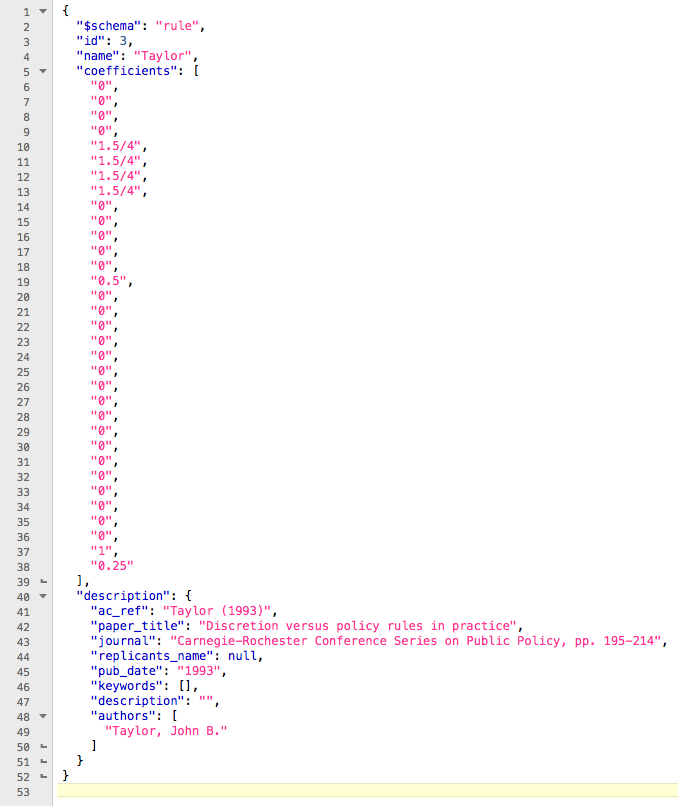
\includegraphics[width=13cm,keepaspectratio]{userrulejson.png}
        \label{img:userruletaylorjson}
        \end{figure}




\noindent {\it 1) Add a common monetary policy rule}\\
%\textbf{TO BE COMPLETED}
\begin{itemize}
%  \item The first task is to choose a suitable name for the new policy rule and to include it into an array for a list of rule names, \emph{rulenames}. One also has to add its acronyms in character arrays, \emph{rulenamesshort} and \emph{rulenamesshort1} \footnote{ As \emph{rulenamesshort1} are used for displaying simulation outcomes in Matlab console, any blank is not allowed in the rule name.}. Please make sure that the new rule name is of the same size of character array as the already existing one. Next, one assigns color to the rule with the array \textit{myrulecolor}.
%	\item Then, one adds the specification of the new-rule coefficients right after the last common rule's specification.
%  \item The remaining work is to add the new rule to the frontend of the MMB 3.0 \\\textbf{TO BE COMPLETED}.
\item In the new version of the MMB, policy rules are entirely defined via json-files. Common policy rules are stored in the subfolder `resources/app/dist/electron/static/mmci-cli/rules'.
\item The first task is to choose a suitable name for the new policy rule and to create a json-file with the same name. This json-file is to be stored in a subfolder with the exactly same name in the \textit{RULE} folder.
\item The json-file for a rule is in general similar to those for models; the whole entry has to be in curly brackets (\{...\}) and blocks are separated by commas. Figure \ref{img:userruletaylorjson} shows an exemplary json-file for the Taylor (1993) rule.
\item First, you have to indicate that the json-file describes a policy rule by setting \texttt{"\$schema": "rule"},
\item Second, you have to give the new rule an id-number by specifying \texttt{"id":\textit{number}}. The number 3 to 11 are already taken by the common policy rules shipped with the MMB.
\item Third, give your rule a name by specifying \texttt{"name": \textit{name}}, which should be the same you have given to the folder and the json-file.
\item Fourth, you have to actually specify the parameters of the rule by setting \texttt{"coefficients": $[$...$]$} to the respective values.
\item Fifth, you need to add a description of the rule, very much like you do in the json-files for models as described in section \ref{sec:ModelfileStructure}. Here, you can set \texttt{"replicants\_name": null}.
\item Safe the json-file and go to the MMB interface, click on `Menu' and `Reload Data'. The new rule should now be displayed under `Policy rules'
\item However, in order to use the new rule for comparison exercises, you also need to add its \texttt{id} to the \texttt{rules} section of all model-jsons for which the rule can/shall be used. This is necessary because not all models can be solved with all parameterizations (see subsection 3 of this chapter) and the new MMB is designed such that only common policy rules can be selected in combination with models in which they actually work. When you have done this, again reload data in the interface. The new rule should now be fully implemented in your MMB.


\end{itemize}


\noindent {\it 2) Add the model-specific monetary policy rule}

\begin{itemize}
  \item When adding a new model, it is possible to include its policy rule as long as the rule can be rewritten in terms of Modelbase common variables. If this is the case, the user should specify the parameters of the model-specific rule in the \texttt{"msr"} section of the model's json-file.
%  add the model identification number to the variable vector \emph{model\_with\_rule} in the  file \emph{MMB\_settings.m} such that a model-specific rule is activated when its corresponding model is chosen in \textbf{Option 2}. Otherwise, the user should add the model number to the variable vector \emph{model\_without\_rule}. For example, if the policy rule is set for the interest rate to react to exchange rate or credit growth, the user cannot include the original rule in the Modelbase.
%  \item Finally, the user has to insert the specification of the model-specific rule into the part of \emph{switch} statement in the file \emph{MMB\_OPTIONS/MSR\_COEFFFS.m} using the model's identification number as the case expression.
\item Reload data in the interface to employ the changes in the MMB.
\end{itemize}

\noindent {\it 3) User-specified monetary rule}

\begin{itemize}
  \item When \textit{User-specified rule} is chosen (see figure \ref{img:PR} in section \ref{sec:usingMMB}), a menu with a general form of a monetary policy rule appears in terms of common variables. Then, one can specify desired coefficient values of each variable in columns and to the corresponding lag/lead in rows.
      For example, to implement the Taylor (1993) rule using the option for user-specified monetary policy rule, one should set the coefficients as following: $ \rho_{\pi,0} = \rho_{\pi,-1} = \rho_{\pi,-2} = \rho_{\pi,-3} = 0.375, \rho_{q,0} = 0.5 $ and the rest of coefficients to zero. Figure \ref{img:userruletaylor} illustrates how to use the option for a user-specified rule with the example of Taylor (1993) rule. \\

        \begin{figure}[H]
        \centering
        \caption{\textsc{Taylor (1993) rule using the option of user-specified rule }}
        \vspace{0.2cm}
        \includegraphics[width=13cm,keepaspectratio]{userrule.png}
        \label{img:userruletaylor}
        \end{figure}

  \item Note that with certain rule parametrization, models cannot be solved due to several reasons. For example, the system of equations may violate the Blanchard-Kahn conditions so a model does not yield a unique stationary rational expectations equilibrium. There is no clear guideline for conditions for determinacy, but \cite{LevinWielandWilliams2003} suggest several crucial characteristics of rules that deliver a unique equilibrium: a relatively short inflation forecast horizon, a moderate degree of responsiveness to the inflation forecast, an explicit response to the current output gap, and a substantial degree of policy inertia.
\end{itemize}


There are three ways to add a new rule to the Modelbase: 1) add a rule to a list of common monetary policy rules, 2) include the model-specific rule calibrated or estimated by the original model authors and 3) specify a rule using the Modelbase user-specified rule option. Below we discuss each case in detail. Keep in mind that policy rules in the Modelbase have to be reformulated in terms of common Modelbase variables such as the annualized quarterly interest rate, the annualized quarter-to-quarter rate of inflation, the quarterly output and the quarterly output gap. This is explained in detail in \cite{WCMSW2012} and in the separate document, called 'MMB\_MPrule\_description.pdf'. 
%Also, one can see how it practically works by looking at common monetary policy rules already implemented in the \emph{MMB\_OPTIONS/MMB\_settings.m} file.
\newline


        \begin{figure}
        \centering
        \caption{\textsc{Taylor (1993) rule as defined in json-file}}
        \vspace{0.2cm}
        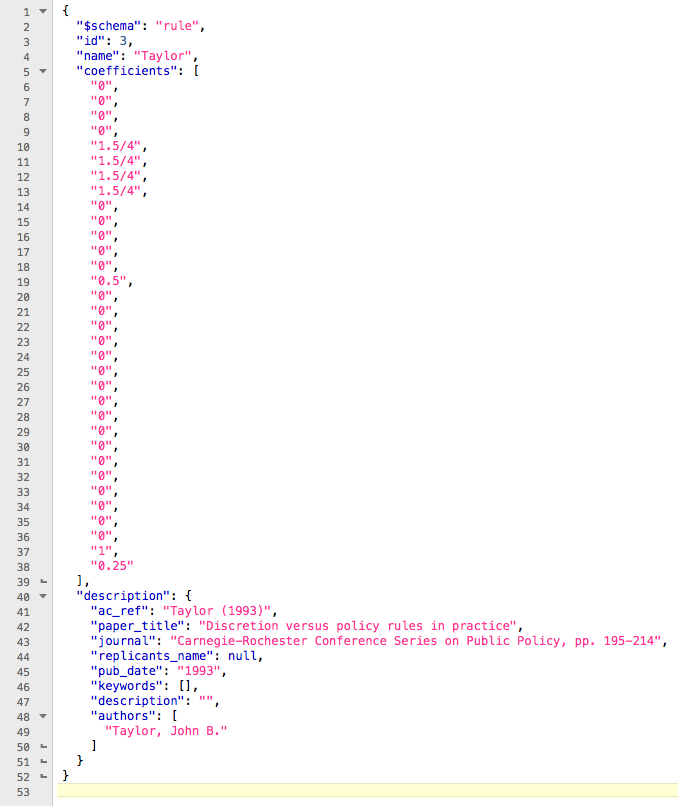
\includegraphics[width=13cm,keepaspectratio]{userrulejson.png}
        \label{img:userruletaylorjson}
        \end{figure}




\noindent {\it 1) Add a common monetary policy rule}\\
%\textbf{TO BE COMPLETED}
\begin{itemize}
%  \item The first task is to choose a suitable name for the new policy rule and to include it into an array for a list of rule names, \emph{rulenames}. One also has to add its acronyms in character arrays, \emph{rulenamesshort} and \emph{rulenamesshort1} \footnote{ As \emph{rulenamesshort1} are used for displaying simulation outcomes in Matlab console, any blank is not allowed in the rule name.}. Please make sure that the new rule name is of the same size of character array as the already existing one. Next, one assigns color to the rule with the array \textit{myrulecolor}.
%	\item Then, one adds the specification of the new-rule coefficients right after the last common rule's specification.
%  \item The remaining work is to add the new rule to the frontend of the MMB 3.0 \\\textbf{TO BE COMPLETED}.
\item In the new version of the MMB, policy rules are entirely defined via json-files. Common policy rules are stored in the subfolder `resources/app/dist/electron/static/mmci-cli/rules'.
\item The first task is to choose a suitable name for the new policy rule and to create a json-file with the same name. This json-file is to be stored in a subfolder with the exactly same name in the \textit{RULE} folder.
\item The json-file for a rule is in general similar to those for models; the whole entry has to be in curly brackets (\{...\}) and blocks are separated by commas. Figure \ref{img:userruletaylorjson} shows an exemplary json-file for the Taylor (1993) rule.
\item First, you have to indicate that the json-file describes a policy rule by setting \texttt{"\$schema": "rule"},
\item Second, you have to give the new rule an id-number by specifying \texttt{"id":\textit{number}}. The number 3 to 11 are already taken by the common policy rules shipped with the MMB.
\item Third, give your rule a name by specifying \texttt{"name": \textit{name}}, which should be the same you have given to the folder and the json-file.
\item Fourth, you have to actually specify the parameters of the rule by setting \texttt{"coefficients": $[$...$]$} to the respective values.
\item Fifth, you need to add a description of the rule, very much like you do in the json-files for models as described in section \ref{sec:ModelfileStructure}. Here, you can set \texttt{"replicants\_name": null}.
\item Safe the json-file and go to the MMB interface, click on `Menu' and `Reload Data'. The new rule should now be displayed under `Policy rules'
\item However, in order to use the new rule for comparison exercises, you also need to add its \texttt{id} to the \texttt{rules} section of all model-jsons for which the rule can/shall be used. This is necessary because not all models can be solved with all parameterizations (see subsection 3 of this chapter) and the new MMB is designed such that only common policy rules can be selected in combination with models in which they actually work. When you have done this, again reload data in the interface. The new rule should now be fully implemented in your MMB.


\end{itemize}


\noindent {\it 2) Add the model-specific monetary policy rule}

\begin{itemize}
  \item When adding a new model, it is possible to include its policy rule as long as the rule can be rewritten in terms of Modelbase common variables. If this is the case, the user should specify the parameters of the model-specific rule in the \texttt{"msr"} section of the model's json-file.
%  add the model identification number to the variable vector \emph{model\_with\_rule} in the  file \emph{MMB\_settings.m} such that a model-specific rule is activated when its corresponding model is chosen in \textbf{Option 2}. Otherwise, the user should add the model number to the variable vector \emph{model\_without\_rule}. For example, if the policy rule is set for the interest rate to react to exchange rate or credit growth, the user cannot include the original rule in the Modelbase.
%  \item Finally, the user has to insert the specification of the model-specific rule into the part of \emph{switch} statement in the file \emph{MMB\_OPTIONS/MSR\_COEFFFS.m} using the model's identification number as the case expression.
\item Reload data in the interface to employ the changes in the MMB.
\end{itemize}

\noindent {\it 3) User-specified monetary rule}

\begin{itemize}
  \item When \textit{User-specified rule} is chosen (see figure \ref{img:PR} in section \ref{sec:usingMMB}), a menu with a general form of a monetary policy rule appears in terms of common variables. Then, one can specify desired coefficient values of each variable in columns and to the corresponding lag/lead in rows.
      For example, to implement the Taylor (1993) rule using the option for user-specified monetary policy rule, one should set the coefficients as following: $ \rho_{\pi,0} = \rho_{\pi,-1} = \rho_{\pi,-2} = \rho_{\pi,-3} = 0.375, \rho_{q,0} = 0.5 $ and the rest of coefficients to zero. Figure \ref{img:userruletaylor} illustrates how to use the option for a user-specified rule with the example of Taylor (1993) rule. \\

        \begin{figure}[H]
        \centering
        \caption{\textsc{Taylor (1993) rule using the option of user-specified rule }}
        \vspace{0.2cm}
        \includegraphics[width=13cm,keepaspectratio]{userrule.png}
        \label{img:userruletaylor}
        \end{figure}

  \item Note that with certain rule parametrization, models cannot be solved due to several reasons. For example, the system of equations may violate the Blanchard-Kahn conditions so a model does not yield a unique stationary rational expectations equilibrium. There is no clear guideline for conditions for determinacy, but \cite{LevinWielandWilliams2003} suggest several crucial characteristics of rules that deliver a unique equilibrium: a relatively short inflation forecast horizon, a moderate degree of responsiveness to the inflation forecast, an explicit response to the current output gap, and a substantial degree of policy inertia.
\end{itemize}


There are three ways to add a new rule to the Modelbase: 1) add a rule to a list of common monetary policy rules, 2) include the model-specific rule calibrated or estimated by the original model authors and 3) specify a rule using the Modelbase user-specified rule option. Below we discuss each case in detail. Keep in mind that policy rules in the Modelbase have to be reformulated in terms of common Modelbase variables such as the annualized quarterly interest rate, the annualized quarter-to-quarter rate of inflation, the quarterly output and the quarterly output gap. This is explained in detail in \cite{WCMSW2012} and in the separate document, called 'MMB\_MPrule\_description.pdf'. 
%Also, one can see how it practically works by looking at common monetary policy rules already implemented in the \emph{MMB\_OPTIONS/MMB\_settings.m} file.
\newline


        \begin{figure}
        \centering
        \caption{\textsc{Taylor (1993) rule as defined in json-file}}
        \vspace{0.2cm}
        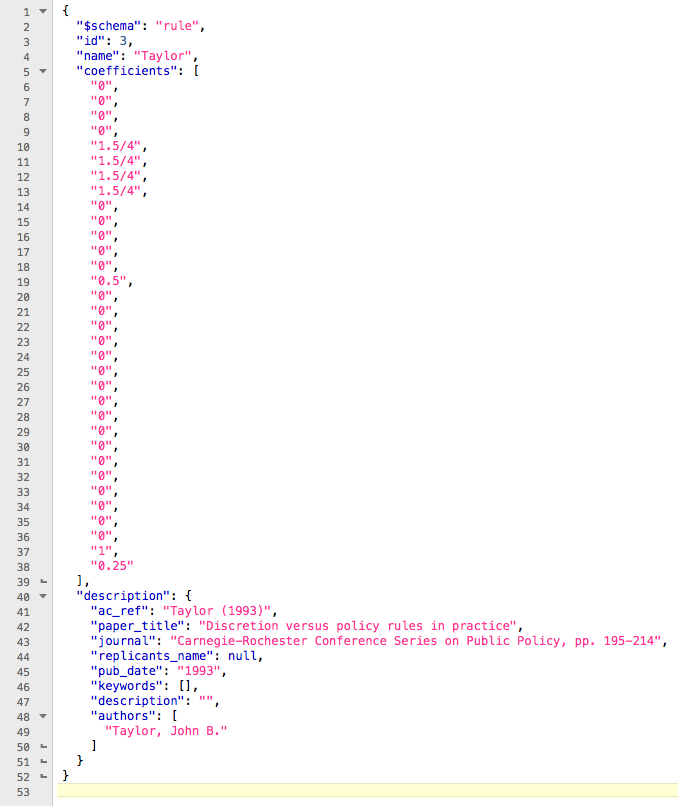
\includegraphics[width=13cm,keepaspectratio]{userrulejson.png}
        \label{img:userruletaylorjson}
        \end{figure}




\noindent {\it 1) Add a common monetary policy rule}\\
%\textbf{TO BE COMPLETED}
\begin{itemize}
%  \item The first task is to choose a suitable name for the new policy rule and to include it into an array for a list of rule names, \emph{rulenames}. One also has to add its acronyms in character arrays, \emph{rulenamesshort} and \emph{rulenamesshort1} \footnote{ As \emph{rulenamesshort1} are used for displaying simulation outcomes in Matlab console, any blank is not allowed in the rule name.}. Please make sure that the new rule name is of the same size of character array as the already existing one. Next, one assigns color to the rule with the array \textit{myrulecolor}.
%	\item Then, one adds the specification of the new-rule coefficients right after the last common rule's specification.
%  \item The remaining work is to add the new rule to the frontend of the MMB 3.0 \\\textbf{TO BE COMPLETED}.
\item In the new version of the MMB, policy rules are entirely defined via json-files. Common policy rules are stored in the subfolder `resources/app/dist/electron/static/mmci-cli/rules'.
\item The first task is to choose a suitable name for the new policy rule and to create a json-file with the same name. This json-file is to be stored in a subfolder with the exactly same name in the \textit{RULE} folder.
\item The json-file for a rule is in general similar to those for models; the whole entry has to be in curly brackets (\{...\}) and blocks are separated by commas. Figure \ref{img:userruletaylorjson} shows an exemplary json-file for the Taylor (1993) rule.
\item First, you have to indicate that the json-file describes a policy rule by setting \texttt{"\$schema": "rule"},
\item Second, you have to give the new rule an id-number by specifying \texttt{"id":\textit{number}}. The number 3 to 11 are already taken by the common policy rules shipped with the MMB.
\item Third, give your rule a name by specifying \texttt{"name": \textit{name}}, which should be the same you have given to the folder and the json-file.
\item Fourth, you have to actually specify the parameters of the rule by setting \texttt{"coefficients": $[$...$]$} to the respective values.
\item Fifth, you need to add a description of the rule, very much like you do in the json-files for models as described in section \ref{sec:ModelfileStructure}. Here, you can set \texttt{"replicants\_name": null}.
\item Safe the json-file and go to the MMB interface, click on `Menu' and `Reload Data'. The new rule should now be displayed under `Policy rules'
\item However, in order to use the new rule for comparison exercises, you also need to add its \texttt{id} to the \texttt{rules} section of all model-jsons for which the rule can/shall be used. This is necessary because not all models can be solved with all parameterizations (see subsection 3 of this chapter) and the new MMB is designed such that only common policy rules can be selected in combination with models in which they actually work. When you have done this, again reload data in the interface. The new rule should now be fully implemented in your MMB.


\end{itemize}


\noindent {\it 2) Add the model-specific monetary policy rule}

\begin{itemize}
  \item When adding a new model, it is possible to include its policy rule as long as the rule can be rewritten in terms of Modelbase common variables. If this is the case, the user should specify the parameters of the model-specific rule in the \texttt{"msr"} section of the model's json-file.
%  add the model identification number to the variable vector \emph{model\_with\_rule} in the  file \emph{MMB\_settings.m} such that a model-specific rule is activated when its corresponding model is chosen in \textbf{Option 2}. Otherwise, the user should add the model number to the variable vector \emph{model\_without\_rule}. For example, if the policy rule is set for the interest rate to react to exchange rate or credit growth, the user cannot include the original rule in the Modelbase.
%  \item Finally, the user has to insert the specification of the model-specific rule into the part of \emph{switch} statement in the file \emph{MMB\_OPTIONS/MSR\_COEFFFS.m} using the model's identification number as the case expression.
\item Reload data in the interface to employ the changes in the MMB.
\end{itemize}

\noindent {\it 3) User-specified monetary rule}

\begin{itemize}
  \item When \textit{User-specified rule} is chosen (see figure \ref{img:PR} in section \ref{sec:usingMMB}), a menu with a general form of a monetary policy rule appears in terms of common variables. Then, one can specify desired coefficient values of each variable in columns and to the corresponding lag/lead in rows.
      For example, to implement the Taylor (1993) rule using the option for user-specified monetary policy rule, one should set the coefficients as following: $ \rho_{\pi,0} = \rho_{\pi,-1} = \rho_{\pi,-2} = \rho_{\pi,-3} = 0.375, \rho_{q,0} = 0.5 $ and the rest of coefficients to zero. Figure \ref{img:userruletaylor} illustrates how to use the option for a user-specified rule with the example of Taylor (1993) rule. \\

        \begin{figure}[H]
        \centering
        \caption{\textsc{Taylor (1993) rule using the option of user-specified rule }}
        \vspace{0.2cm}
        \includegraphics[width=13cm,keepaspectratio]{userrule.png}
        \label{img:userruletaylor}
        \end{figure}

  \item Note that with certain rule parametrization, models cannot be solved due to several reasons. For example, the system of equations may violate the Blanchard-Kahn conditions so a model does not yield a unique stationary rational expectations equilibrium. There is no clear guideline for conditions for determinacy, but \cite{LevinWielandWilliams2003} suggest several crucial characteristics of rules that deliver a unique equilibrium: a relatively short inflation forecast horizon, a moderate degree of responsiveness to the inflation forecast, an explicit response to the current output gap, and a substantial degree of policy inertia.
\end{itemize}




%\appendix
%\numberwithin{table}{section}
%\cleardoublepage
%\addcontentsline{toc}{section}{References}

%\nocite{*}
\bibliographystyle{elsarticle-harv}
\bibliography{DynareModelBase}

\end{document}
